\documentclass[output=book
		,modfonts
		,nonflat
	        ,collection
	        ,collectionchapter
	        ,collectiontoclongg
 	        ,biblatex  
                ,babelshorthands
%                ,showindex
                ,newtxmath
                ,colorlinks, citecolor=brown 
                ,draftmode
% 	        ,coverus
		  ]{./langsci/langscibook}                              
%%%%%%%%%%%%%%%%%%%%%%%%%%%%%%%%%%%%%%%%%%%%%%%%%%%%

% put all additional commands you need in the 
% following files. If you do not know what this might 
% mean, you can safely ignore this section

\title{The one and only handbook of Head-Driven Phrase Structure Grammar}  %look no further, you can change those things right here.
\subtitle{}
% \BackTitle{Change your backtitle in localmetadata.tex} % Change if BackTitle != Title
\BackBody{change blurb in localmetadata.tex
 }
%\dedication{Change dedication in localmetadata.tex}
%\typesetter{Change typesetter in localmetadata.tex}
%\proofreader{Change proofreaders in localmetadata.tex}
\author{Anne Abeillé\and Robert D. Bors­ley\and Jean-​Pierre Koenig\lastand Stefan Müller}
% \BookDOI{}%ask coordinator for DOI
\renewcommand{\lsISBNdigital}{000-0-000000-00-0}
\renewcommand{\lsISBNhardcover}{000-0-000000-00-0}
\renewcommand{\lsISBNsoftcover}{000-0-000000-00-0}
\renewcommand{\lsISBNsoftcoverus}{000-0-000000-00-0}
\renewcommand{\lsSeries}{eotms} % use lowercase acronym, e.g. sidl, eotms, tgdi
\renewcommand{\lsSeriesNumber}{99} %will be assigned when the book enters the proofreading stage
% \renewcommand{\lsURL}{http://langsci-press.org/catalog/book/000} % contact the coordinator for the right number

% add all extra packages you need to load to this file 

\usepackage{graphicx}
\usepackage{tabularx}
\usepackage{amsmath} 
\usepackage{multicol}
\usepackage{lipsum}
%%%%%%%%%%%%%%%%%%%%%%%%%%%%%%%%%%%%%%%%%%%%%%%%%%%%
%%%                                              %%%
%%%           Examples                           %%%
%%%                                              %%%
%%%%%%%%%%%%%%%%%%%%%%%%%%%%%%%%%%%%%%%%%%%%%%%%%%%%
% remove the percentage signs in the following lines
% if your book makes use of linguistic examples


\usepackage{./langsci/styles/langsci-gb4e} 
\usepackage{./langsci/styles/langsci-optional} 
\usepackage{./langsci/styles/langsci-lgr}
\usepackage{./langsci/styles/langsci-forest-setup}
\usepackage{morewrites}



% Stefan Müller's styles
\usepackage{./styles/merkmalstruktur,./styles/abbrev,./styles/makros.2e,./styles/my-xspace,./styles/article-ex,
./styles/eng-date}

\usepackage{./langsci/styles/jambox}

% Crossing out text
% uncomment when needed
%\usepackage{ulem}

\usepackage{./styles/additional-langsci-index-shortcuts}

\usepackage{./styles/avm+}

\renewcommand{\tpv}[1]{{\avmjvalfont\itshape #1}}

\regAvmFonts

\usepackage{theorem}

\newtheorem{mydefinition}{Def.}
\newtheorem{principle}{Principle}

{\theoremstyle{break}
\newtheorem{schema}{Schema}
\newtheorem{mydefinition-break}[mydefinition]{Def.}
\newtheorem{principle-break}[principle]{Principle}
}

\usepackage{subfig}

%% hyphenation points for line breaks
%% Normally, automatic hyphenation in LaTeX is very good
%% If a word is mis-hyphenated, add it to this file
%%
%% add information to TeX file before \begin{document} with:
%% %% hyphenation points for line breaks
%% Normally, automatic hyphenation in LaTeX is very good
%% If a word is mis-hyphenated, add it to this file
%%
%% add information to TeX file before \begin{document} with:
%% %% hyphenation points for line breaks
%% Normally, automatic hyphenation in LaTeX is very good
%% If a word is mis-hyphenated, add it to this file
%%
%% add information to TeX file before \begin{document} with:
%% \include{localhyphenation}
\hyphenation{
A-la-hver-dzhie-va
anaph-o-ra
affri-ca-te
affri-ca-tes
Atha-bas-kan
com-ple-ments
Da-ge-stan
Dor-drecht
er-klä-ren-de
Ginz-burg
Gro-ning-en
Jon-a-than
Ka-tho-lie-ke
Ko-bon
krie-gen
Le-Sourd
moth-er
Mül-ler
Nie-mey-er
Prze-piór-kow-ski
phe-nom-e-non
re-nowned
Rie-he-mann
un-bound-ed
}

% why has "erklärende" be listed here? I specified langid in bibtex item. Something is still not working with hyphenation.


% to do: check
%  Alahverdzhieva

\hyphenation{
A-la-hver-dzhie-va
anaph-o-ra
affri-ca-te
affri-ca-tes
Atha-bas-kan
com-ple-ments
Da-ge-stan
Dor-drecht
er-klä-ren-de
Ginz-burg
Gro-ning-en
Jon-a-than
Ka-tho-lie-ke
Ko-bon
krie-gen
Le-Sourd
moth-er
Mül-ler
Nie-mey-er
Prze-piór-kow-ski
phe-nom-e-non
re-nowned
Rie-he-mann
un-bound-ed
}

% why has "erklärende" be listed here? I specified langid in bibtex item. Something is still not working with hyphenation.


% to do: check
%  Alahverdzhieva

\hyphenation{
A-la-hver-dzhie-va
anaph-o-ra
affri-ca-te
affri-ca-tes
Atha-bas-kan
com-ple-ments
Da-ge-stan
Dor-drecht
er-klä-ren-de
Ginz-burg
Gro-ning-en
Jon-a-than
Ka-tho-lie-ke
Ko-bon
krie-gen
Le-Sourd
moth-er
Mül-ler
Nie-mey-er
Prze-piór-kow-ski
phe-nom-e-non
re-nowned
Rie-he-mann
un-bound-ed
}

% why has "erklärende" be listed here? I specified langid in bibtex item. Something is still not working with hyphenation.


% to do: check
%  Alahverdzhieva

%add all your local new commands to this file

\makeatletter
\def\blx@maxline{77}
\makeatother 


% udc stuff
\newcommand{\tnode}[2]{
 \rnode{#1}{\emph{#2}}
}

\newcommand{\bcdiag}[2]{
  \ncdiag{#1}{#2}
}


%%%%%%%%%%%%%%%%%%%%%%%%%%%%%%%%%%%%%%%%%%%%%%%%%%%% 
%%%             Frontmatter                      %%% 
%%%%%%%%%%%%%%%%%%%%%%%%%%%%%%%%%%%%%%%%%%%%%%%%%%%%
\begin{document}         
\maketitle                
\frontmatter

\currentpdfbookmark{Contents}{name} % adds a PDF bookmark
%%
\mainmatter          

{\avmoptions{center}


%%%%%%%%%%%%%%%%%%%%%%%%%%%%%%%%%%%%%%%%%%%%%%%%%%%% 
%%%             Chapters                         %%% 
%%%%%%%%%%%%%%%%%%%%%%%%%%%%%%%%%%%%%%%%%%%%%%%%%%%%

% Uncomment the chapter(s) you would like to check

\begin{forest}
[{\footnotesize\textit{object}}
[{{\avmoptions{center}\begin{avm}\[\asort{substantive}
						prd & boolean\]\end{avm}}}
  [{{\avmoptions{center}\begin{avm}\[\asort{verb} vform & vform\\
                                                  prd & plus\]\end{avm}}}]
  [{{\avmoptions{center}\begin{avm}\[\asort{noun} case & case\]\end{avm}}}] ]
[{\footnotesize\textit{case}}]
[{\footnotesize\textit{vform}}]
[{\footnotesize\textit{boolean}}
  [{\footnotesize\textit{plus}}]
  [{\footnotesize\textit{minus}}] ]
]
\end{forest}



\begin{forest}
[{\footnotesize\textit{list}}
  [{{\avmoptions{center}\begin{avm}\[\asort{nelist} first & object\\
                                                    rest & list\]\end{avm}}}]
  [{\footnotesize\textit{elist}} ]]
    \end{forest}

\oneline{%

	\begin{forest}
		[{\type{univ-pas-bas-lci}}
		[{\type{univ-do-pas-lci}}, name=D
		[{\type{german-zuinf-pas-lci}}, name=Z
		[{\type{german-pers-zuinf-pas-lci}} 
		[{\type{german-long-pers-neutral-zuinf-pas-lci}}, name=PZ
		[{\type{german-long-pers-zuinf-pas-lci}} ]
		[{\type{german-long-attr-zuinf-pas-lci}} ]
		]		
		]
		]
		]
		[{\type{german-pas-lci}}, name=G
		[ , no edge ]
		[{\type{german-long-pas-lci}}, name=L
		[ , no edge ]  ]
		[{\type{german-io-pas-lci}} ]	
		]
		[ {\type{univ-imp-pas-lci}} ]
		[ {\ldots} ]
		]
		\draw(G.south) -- (Z.north); 
		\draw(L.south) -- (PZ.north);
	\end{forest}}


\begin{forest}
[{\type{head}}
[{\type{func}}  [{\type{det}} ] [{\type{marker}} ] ]
[{\type{subst}} [{\type{noun}} 
					[{\type{c-noun}} ] [{\type{gerund}}, name=G ]
				  ]
				 [{\type{relational}}, name=R
				 [, no edge ] 
				 [{\type{verb}} ] [{\type{adj}} ] [{\type{prep}} ]
				 ] ]
]
\draw(R.south) -- (G.north);
\end{forest}


	\begin{forest}
       [{\type{verb}} 
      					[{\fbox{\attrib{vform}}}
      						[{\type{fin}}, name=A1  
      						 [{\tc{gray}{\type{fin+intrans}}}, name=A,edge={gray,dashed}   ]    		
      							[, no edge ] ]
      						[{\type{base}}, name=B1       							[{\tc{gray}{\type{base+trans}}}, name=B,
      								edge={gray,dashed}  ]   		 
      							[, no edge ] ]
      						] 
      					[{\fbox{\attrib{arg-st}}} 
      					    [{\type{intrans}}, name=C1 
      					 		[, no edge ]
      					 		[{\tc{gray}{\type{base+intrans}}}, name=C,edge={gray,dashed}  ] ]
      						[{\type{trans}}, name=D1 
      						     [, no edge ]
      						     [{\tc{gray}{\type{fin+trans}}}, name=D,edge={gray,dashed} ]   ]
      					]  
      	]
      				\draw[style=dashed,gray] (C1.south) -- (A.north);
      				\draw[style=dashed,gray] (D1.south)-- (B.north);
      				\draw[style=dashed,gray] (B1.south)-- (C.north);
      				\draw[style=dashed,gray] (A1.south)-- (D.north);
\end{forest}

\oneline{%
\begin{forest}
for tree={inner sep=-1pt,l=50pt}
[{\type{aller}}
  [{\fbox{\type{aller-entries}}}
	[{\type{``fit}}, name=F
		 [{\tc{gray}{\type{``fit''+all-}}}, name=F1,edge={dashed,gray},tier=bottom ]
		 [{\tc{gray}{\type{``fit''+v-}}}, name=F2,edge={dashed,gray},tier=bottom ]
		 [, no edge ]  
		 [, no edge ] ]
	[{\type{``go''}}
		[{\type{``go.to''}}, name=G
			[{\tc{gray}{\type{``go.to''+all-}}}, name=G1, edge={dashed,gray} ]
			[{\tc{gray}{\type{``go.to''+v-}}}, name=G2, edge={dashed,gray} ]
			[, no edge ]
			[, no edge ] ]
		[{\type{``leave''}}, name=L, for tree={l=100pt}
			[{\tc{gray}{\type{``leave''+all-}}}, name=L1,edge={dashed,gray} ]
			[{\tc{gray}{\type{``leave''+v-}}}, name=L2,edge={dashed,gray} ]
			[, no edge ] 
			[, no edge ] 
			 ] ]
	]
  [{\fbox{\type{aller-stems}}}, for tree={l=100pt,inner sep=-3pt} 
  	[{\type{all-}}, name=A
  		[, no edge ]
		[, no edge ]
		[, no edge ]
  	]
  	[{\type{v-}}, name=V
  		[, no edge ]
		[, no edge ]
		[, no edge ]
  	]
  	[{\type{i-}}, name=I, for tree={l=80pt} 
		[{\tc{gray}{\type{``fit''+i-}}}, name=I1,edge={dashed,gray} ]
		[{\tc{gray}{\type{``go.to''+i-}}}, name=I2,edge={dashed,gray} ]
		[{\tc{gray}{\type{``leave''+i-}}},  name=I3,edge={dashed,gray} ]
  	]
  	[{\type{aill-}}, name=AI, for tree={l=100pt,inner sep=-3pt}
  		[{\tc{gray}{\type{``fit''+aill-}}}, name=A1, edge={dashed,gray} ]
		[{\tc{gray}{\type{``go.to''+aill-}}}, name=A2, edge={dashed,gray} ]
		[{\tc{gray}{\type{``leave''+aill-}}}, name=A3, edge={dashed,gray},tier=bottom ]  	
	]
  ]
]
\draw[style=dashed,gray](A.south) -- (F1.north); 
\draw[style=dashed,gray](V.south) -- (F2.north); 
\draw[style=dashed,gray](A.south) -- (G1.north); 
\draw[style=dashed,gray](V.south) -- (G2.north); 
\draw[style=dashed,gray](A.south) -- (L1.north); 
\draw[style=dashed,gray](V.south) -- (L2.north); 
\draw[style=dashed,gray](F.south) -- (I1.north);
\draw[style=dashed,gray](F.south) -- (A1.north);
\draw[style=dashed,gray](G.south) -- (I2.north);
\draw[style=dashed,gray](G.south) -- (A2.north);
\draw[style=dashed,gray](L.south) -- (I3.north);
\draw[style=dashed,gray](L.south) -- (A3.north);
\end{forest}}

\hspace*{-1em}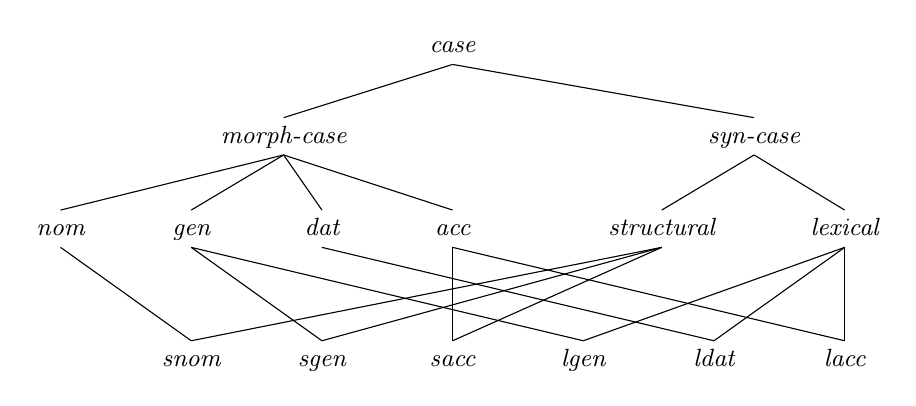
\begin{tikzpicture}[text height=1.5ex,text depth=.25ex,
  % inner sep=2pt,
  node distance=5em,
  baseline=10.75em]\small\it
\node (snom) {snom};
\node (sgen) [right of=snom] {sgen};
\node (sacc) [right of=sgen] {sacc};
\node (lgen) [right of=sacc] {lgen};
\node (ldat) [right of=lgen] {ldat};
\node (lacc) [right of=ldat] {lacc};
\node (acc) [above of=sacc] {acc};
\node (dat) [left of=acc] {dat};
\node (gen) [left of=dat] {gen};
\node (nom) [left of=gen] {nom};
\node (structural) [above of=lgen, xshift=3em] {structural};
\node (lexical) [above of=lacc] {lexical};
\node (morph-case) [above right of=gen] {morph-case};
\node (syn-case) [above right of=structural] {syn-case};
\node (case) [above of=acc, node distance=7em] {case};
\draw (case.south) -- (morph-case.north);
\draw (case.south) -- (syn-case.north);
\draw (morph-case.south) -- (nom.north);
\draw (morph-case.south) -- (gen.north);
\draw (morph-case.south) -- (dat.north);
\draw (morph-case.south) -- (acc.north);
\draw (syn-case.south) -- (structural.north);
\draw (syn-case.south) -- (lexical.north);
\draw (nom.south) -- (snom.north);
\draw (gen.south) -- (sgen.north);
\draw (gen.south) -- (lgen.north);
\draw (dat.south) -- (ldat.north);
\draw (acc.south) -- (sacc.north);
\draw (acc.south) -- (lacc.north);
\draw (structural.south) -- (snom.north);
\draw (structural.south) -- (sgen.north);
\draw (structural.south) -- (sacc.north);
\draw (lexical.south) -- (lgen.north);
\draw (lexical.south) -- (ldat.north);
\draw (lexical.south) -- (lacc.north);
\end{tikzpicture}


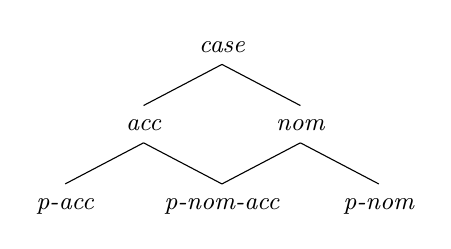
\begin{tikzpicture}[text height=1.5ex,text depth=.25ex,
  % inner sep=2pt,
  node distance=3em,
  baseline=5.25em]\small\it
\node (p-acc) {p-acc};
\node (p-acc1) [right of=p-acc] {};
\node (p-nom-acc) [right of=p-acc1] {p-nom-acc};
\node (p-nom1) [right of=p-nom-acc] {};
\node (p-nom) [right of=p-nom1] {p-nom};
\node (acc) [above of=p-acc1] {acc};
\node (nom) [above of=p-nom1] {nom};
\node (p-nom-acc1) [above of=p-nom-acc] {};
\node (case) [above of=p-nom-acc1] {case};
\draw (case.south) -- (acc.north);
\draw (case.south) -- (nom.north);
\draw (acc.south) -- (p-acc.north);
\draw (acc.south) -- (p-nom-acc.north);
\draw (nom.south) -- (p-nom.north);
\draw (nom.south) -- (p-nom-acc.north);
\end{tikzpicture}

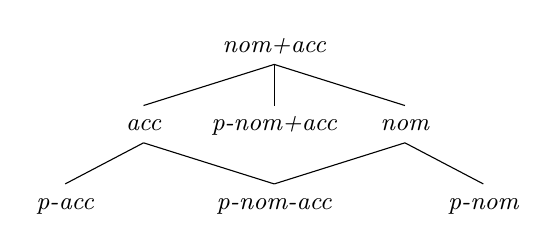
\begin{tikzpicture}[text height=1.5ex,text depth=.25ex,
  % inner sep=2pt,
  node distance=4em,
  baseline=5.25em]\small\it
\node (p-acc) {p-acc};
\node (p-acc1) [right of=p-acc] {};
\node (p-nom-acc) [right of=p-acc1] {p-nom-acc};
\node (p-nom1) [right of=p-nom-acc] {};
\node (p-nom) [right of=p-nom1] {p-nom};
\node (acc) [above of=p-acc1, node distance=3em, xshift=-1em] {acc};
\node (nom) [above of=p-nom1, node distance=3em, xshift=1em] {nom};
\node (p-nom+acc) [above of=p-nom-acc, node distance=3em] {p-nom+acc};
\node (nom+acc) [above of=p-nom+acc, node distance=3em] {nom+acc};
\draw (nom+acc.south) -- (acc.north);
\draw (nom+acc.south) -- (nom.north);
\draw (nom+acc.south) -- (p-nom+acc.north);
\draw (acc.south) -- (p-acc.north);
\draw (acc.south) -- (p-nom-acc.north);
\draw (nom.south) -- (p-nom.north);
\draw (nom.south) -- (p-nom-acc.north);
\end{tikzpicture}


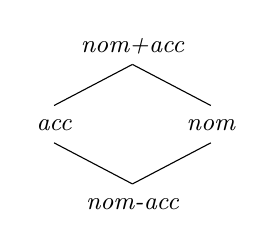
\begin{tikzpicture}[text height=1.5ex,text depth=.25ex,
  % inner sep=2pt,
  node distance=3em,
  baseline=2.5em]\small\it
\node (acc) {acc};
\node (accnom) [right of=acc] {};
\node (nom) [right of=accnom] {nom};
\node (nom-acc) [below of=accnom] {nom-acc};
\node (nom+acc) [above of=accnom] {nom+acc};
\draw (nom+acc.south) -- (acc.north);
\draw (nom+acc.south) -- (nom.north);
\draw (acc.south) -- (nom-acc.north);
\draw (nom.south) -- (nom-acc.north);
\end{tikzpicture}



\hfill\hfill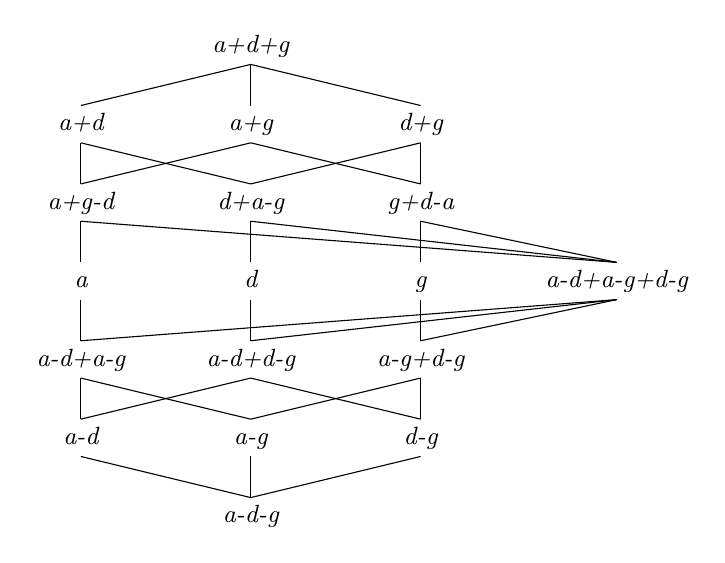
\begin{tikzpicture}[text height=1.5ex,text depth=.25ex,
  % inner sep=2pt,
  node distance=6.5em,
  baseline=8em]\small\it
\node (a) {a};
\node (d) [right of=a] {d};
\node (g) [right of=d] {g};
\node (a-d+a-g+d-g) [right of=g, xshift=1em] {a-d+a-g+d-g};
\node (a+g-d) [above of=a, node distance=3em]  {a+g-d};
\node (d+a-g) [above of=d, node distance=3em] {d+a-g};
\node (g+d-a) [above of=g, node distance=3em] {g+d-a};
\node (a+d) [above of=a+g-d, node distance=3em] {a+d};
\node (a+g) [above of=d+a-g, node distance=3em] {a+g};
\node (d+g) [above of=g+d-a, node distance=3em] {d+g};
\node (a+d+g) [above of=a+g, node distance=3em] {a+d+g};
\node (a-d+a-g) [below of=a, node distance=3em] {a-d+a-g};
\node (a-d+d-g) [below of=d, node distance=3em] {a-d+d-g};
\node (a-g+d-g) [below of=g, node distance=3em] {a-g+d-g};
\node (a-d) [below of=a-d+a-g, node distance=3em] {a-d};
\node (a-g) [below of=a-d+d-g, node distance=3em] {a-g};
\node (d-g) [below of=a-g+d-g, node distance=3em] {d-g};
\node (a-d-g) [below of=a-g, node distance=3em] {a-d-g};
\draw (a+g-d.south) -- (a.north);
\draw (a+g-d.south) -- (a-d+a-g+d-g.north);
\draw (d+a-g.south) -- (d.north);
\draw (d+a-g.south) -- (a-d+a-g+d-g.north);
\draw (g+d-a.south) -- (g.north);
\draw (g+d-a.south) -- (a-d+a-g+d-g.north);
\draw (a+d.south) -- (a+g-d.north);
\draw (a+d.south) -- (d+a-g.north);
\draw (a+g.south) -- (a+g-d.north);
\draw (a+g.south) -- (g+d-a.north);
\draw (d+g.south) -- (d+a-g.north);
\draw (d+g.south) -- (g+d-a.north);
\draw (a+d+g.south) -- (a+d.north);
\draw (a+d+g.south) -- (a+g.north);
\draw (a+d+g.south) -- (d+g.north);
\draw (a.south) -- (a-d+a-g.north);
\draw (d.south) -- (a-d+d-g.north);
\draw (g.south) -- (a-g+d-g.north);
\draw (a-d+a-g.south) -- (a-d.north);
\draw (a-d+a-g.south) -- (a-g.north);
\draw (a-d+d-g.south) -- (a-d.north);
\draw (a-d+d-g.south) -- (d-g.north);
\draw (a-g+d-g.south) -- (a-g.north);
\draw (a-g+d-g.south) -- (d-g.north);
\draw (a-d.south) -- (a-d-g.north);
\draw (a-g.south) -- (a-d-g.north);
\draw (d-g.south) -- (a-d-g.north);
\draw (a-d+a-g+d-g.south) -- (a-d+a-g.north);
\draw (a-d+a-g+d-g.south) -- (a-d+d-g.north);
\draw (a-d+a-g+d-g.south) -- (a-g+d-g.north);
\end{tikzpicture}\hfill\mbox{}



\begin{forest}
%sm edges
[\type{phrase}
	[\textsc{headedness}
		[\type{headed-phrase}
			[\type{head-subject-phrase} [\type{nonfin-head-subj-cx}, name=A2]]
                        [...]			
                        [\type{head-spr-phrase} [\type{noun-poss-cx}, name=B2]]]]			
	[\textsc{clausality}
		[\type{clause}, name=A1]
		[\type{non-clause}, name=B1]]]
\draw (A1.south) -- (A2.north);
\draw (B1.south) -- (B2.north);
\end{forest}



\begin{forest}
%sm edges
[\type{phrase}
	[\textsc{headedness}
		[\type{headed-phrase}
			[\type{head-nonargument-phrase}
				[\type{head-functor-phr} [\type{regular-nominal-phrase}, name=B2]]
				[\type{head-independent-phr}, name=A1]]]]
	[\textsc{clausality}
		[\type{non-clause}
			[\type{nominal-parameter}
			[\type{intersective-modification}, name=B1 [\type{big-mess-phrase}, name=A2]]]]]]
\draw (A1.south) -- (A2.north);
\draw (B1.south) -- (B2.north);
\end{forest}


	\begin{forest}
       [{\type{lexeme}} 
      					[{\fbox{\attrib{part-of-speech}}}
      						[{\type{verb-lx}}, name=A1 
      							[, no edge ]
      							[, no edge ] ] 
      						 [{\type{adj-lx}}]
      						 [{\type{noun-lx}}] 
      						 [{\ldots}]   		
      					] 
      					[{\fbox{\attrib{arg-selection}}} 
      					    [{\type{intr-lx}}
      					 		[{\type{subj-rsg-lx}}
      					 			[{\type{srv-lx}}, name=B1 ]
      					 		]
      					 		[{\ldots}]
      					 	]
      					 	 [{\type{tr-lx}}
      					 		[{\type{obj-rsg-lx}}
      					 			[{\type{orv-lx}}, name=B2 ]
      					 		]
      					 		[{\ldots}]
      					 	]
      					 	[{\ldots}]
      					]  
      	]
      	\draw (A1.south)-- (B1.north);
      	\draw (B2) to [bend left= 6] (A1);
\end{forest}





\begin{tabular}{cccc}
  \tnode{hf}{head-filler-ph} & \tnode{itrr}{interr-cl} & \tnode{rel}{rel-cl} & \tnode{decl}{decl-cl}\\[2em]

  \tnode{whi}{wh-interr-cl} & \tnode{whr}{wh-rel-cl} & \tnode{top}{top-cl} & \tnode{the}{the-cl}
\end{tabular}



\psset{linewidth=.5pt,angleA=-90,angleB=90,arm=0pt,nodesepA=2pt}

\bcdiag{hf}{whi}
\bcdiag{itrr}{whi}
\bcdiag{hf}{whr}
\bcdiag{rel}{whr}
\bcdiag{hf}{top}
\bcdiag{decl}{top}
\bcdiag{hf}{the}
\bcdiag{decl}{the}

\begin{tabular}{ccccc}
\multicolumn{2}{c}{\tnode{hf}{head-filler-ph}} & \tnode{itrr}{interr-cl} & \tnode{rel}{rel-cl} & \tnode{decl}{decl-cl}\\[1em]
\tnode{std}{standard-head-fill-ph}\\[1.5em]
\tnode{whi}{wh-interr-cl} & \multicolumn{2}{c}{\tnode{whr}{wh-rel-cl}} & \tnode{top}{top-cl} & \tnode{the}{the-cl}\\[1.5em]
&  \tnode{fwh}{fin-wh-rel-cl} & \tnode{iwh}{inf-wh-rel-cl}


\end{tabular}



\psset{linewidth=.5pt,angleA=-90,angleB=90,arm=0pt,nodesepA=2pt}
  
\bcdiag{hf}{std}
\bcdiag{std}{whi}
\bcdiag{itrr}{whi}
\bcdiag{std}{whr}
\bcdiag{rel}{whr}
\bcdiag{std}{top}
\bcdiag{decl}{top}
\bcdiag{hf}{the}
\bcdiag{decl}{the}
\bcdiag{whr}{fwh}
\bcdiag{whr}{iwh}


  \includegraphics[scale=1.2]{figures/Riehemann-crop.pdf}


  \includegraphics[scale=.84]{figures/OTC-crop.pdf}

  \includegraphics[scale=.63]{figures/pretyping-crop.pdf}



\begin{forest}
[\emph{verb-infl}
	[2ND-SLOT,draw
    	[\emph{1sg},name=1sg
    		[\emph{1sg-pos}]
    	]
    	[\emph{3pl}]
   ]
	[1ST-SLOT,draw
		[\emph{neg}
			[\emph{1sg-neg},name=neg]
			[\emph{¬1sg-neg}]
		]
		[\emph{pos}]
	]
	[3RD-SLOT,draw
		[\emph{pst}
			[\emph{pos-pst}]
			[\emph{neg-pst}]
		]
		[\emph{fut}]
	]
]
\draw (1sg.south) to (neg.north);
\end{forest}



%% This does not compile ....

\scalebox{.8}{%
\begin{forest}for tree={l=2cm}
[\emph{realisation-rule}
	[MORPHOTACTICS,draw, name=morph
		[{\begin{avm}
			\[
			mud & \{\normalfont\textit{agr} \}\\
			ms & \{ \[\asort{pid}
			cat & verb\], ...\}\\
			mph & \< \[pc & $-4$\]\> \]
		\end{avm}}, name= 1, tier=word]
		[{\begin{avm}
			\[mud & \{\normalfont\textit{agr}\}\\
			 ms & \{ \[\asort{pid}
			cat & \[\asort{adj}
			type & A\]\], ...\}\\
			mph & \< \[pc & -1\]\>\]
		\end{avm}}, name=2, tier=word]
	]
	[EXPONENCE,draw
		[QUAL,draw, name=qual
			[{\begin{avm}
				\[mud & \{ \[\normalfont\textit{agr}\\cl & 7\]\}\\
				mph & \< ... \[ph & \<\normalfont ca\>\\
				pc & $-1$ $\vee$ $-2$
				\] ... \>\]
			\end{avm}}, tier=word]
			[\dots]
		]
		[CONC,draw, name=conc
			[{\begin{avm}
				\[mud & \{ \[\normalfont\textit{agr}\\cl & 7\]\}\\
				mph & \< ... \[ph & \<\normalfont ci\>\\
				pc & $-1$ $\vee$ $-4$
				\] ... \>\]
			\end{avm}}, tier=word]
			[\dots]
		]
	]
]
%% sorry this is an ugly workaround but even on stackexchange, no one could help me :/
\node[below of=morph, node distance= 8cm](3){%
	{\begin{avm}
			\[mud & \{\normalfont\textit{agr}\}\\
			ms & \{ \[\asort{pid}
			cat & \[\asort{adj}
			type & B\]\], ...\}\\
			mph & \<\[pc & $-2$\], \[pc & $-1$\]\>\]
	\end{avm}}%
};
\draw (1.north) to (qual.south);
\draw (2.north) to (conc.south);
\draw (3.north) to (morph.south);
\end{forest}
}    


  \begin{tabular}{lcc}
    \rnode{u1}{\textsc{beak}} & \rnode{u2}{\textsc{gen}} & \rnode{u3}{\textsc{pl}}\\[2ex]
    \rnode{l1}{nokk} & \rnode{l2}{-a} & \rnode{l3}{-de}
  \end{tabular}
      \psset{angleA=-90,angleB=90,arm=0pt,linewidth=.5pt}

      \ncdiag{u1}{l1} \ncdiag{u1}{l2} \ncdiag{u2}{l1} \ncdiag{u2}{l3}
      \ncdiag{u3}{l1} \ncdiag{u3}{l2} \ncdiag{u3}{l3}


\begin{forest}
[\emph{realisation-rule}
	[SHAPE,draw
		[{\begin{avm}
			\[ mph & \{\[ph &  \<\normalfont ni\>\]\}\\
			mud & \{\[per & 1\\ num & sg\]\}
			\]
		\end{avm}}, name=1
			[{\begin{avm}
				\[ mph & \{\[ph &  \<\normalfont ni\>\\ pc & 2\]\}\\
				mud & \{ \[\asort{subj} per & 1\\ num & sg\] \}
				\]
			\end{avm}}, name=a, no edge, tier=word, l=3cm]
		]
		[{\begin{avm}
			\[ mph & \{\[ph &  \<\normalfont wa\>\]\}\\
			mud & \{\[per & 3\\ num & pl\]\}
			\]
		\end{avm}}, name=2
			[{\begin{avm}
				\[ mph & \{\[ph &  \<\normalfont wa\>\\ pc & 5\]\}\\
				mud & \{ \[\asort{obj} per & 3\\ num & pl\] \}
				\]
			\end{avm}}, name=b, no edge, tier=word, l=3cm]
		]
	]
	[POSITION,draw
		[{\begin{avm}
			\[ mph & \{\[pc & 2\]\}\\
			mud & \{subj\}
			\]
		\end{avm}}, name=3
			[{\begin{avm}
				\[ mph & \{\[ph &  \<\normalfont wa\>\\ pc & 2\]\}\\
				mud & \{ \[\asort{subj} per & 3\\ num & pl\] \}
				\]
			\end{avm}}, name=c, no edge, tier=word, l=3cm]
		]
		[{\begin{avm}
			\[ mph & \{\[pc & 5\]\}\\
			mud & \{ obj \}
			\]
		\end{avm}}, name=4
			[{\begin{avm}
				\[ mph & \{\[ph &  \<\normalfont ni\>\\ pc & 5\]\}\\
				mud & \{\[\asort{obj} per & 1\\ num & sg\]\}
				\]
			\end{avm}}, name=d, no edge, tier=word, l=3cm]
		]
	]
]
\draw[dashed] (1.south) to (a.north);
\draw[dashed] (1.south) to (d.north);
\draw[dashed] (2.south) to (b.north);
\draw[dashed] (2.south) to (c.north);
\draw[dashed] (3.south) to (c.north);
\draw[dashed] (3.south) to (a.north);
\draw[dashed] (4.south) to (b.north);
\draw[dashed] (4.south) to (d.north);
\end{forest}






}


\end{document} 

%%%%%%%%%%%%%%%%%%%%%%%%%%%%%%%%%%%%%%%%%%%%%%%%%%%% 
%%%                  END                         %%% 
%%%%%%%%%%%%%%%%%%%%%%%%%%%%%%%%%%%%%%%%%%%%%%%%%%%% 
